\title{Test Case 2 - Fluids Labs}
\author{
        Sergio M. Vanegas A.\\
                Department of Mathematics\\
        Polimi---Politecnico di Milano\\
        Milano, Italia
}
\date{\today}

\documentclass[12pt]{article}

\usepackage{amsmath}
\usepackage{graphicx}
\usepackage{siunitx}

\begin{document}
\maketitle

\begin{abstract}
        The present case concerns the development of the turbulent flow between two parallel plates. The flow develops from a condition of uniform velocity (rectangular profile) imposed at the inlet boundary, reaching a fully-developed state at a certain distance from the inlet, and it does not change further downstream until the outlet section. Unlike that in the laminar regime (plane Poiseuille flow), the turbulent flow between two parallel plates does not have any analytical solution. In this laboratory, PHOENICS is used to simulate the flow by solving the RANS coupled with the \( k \text{-} \epsilon\) standard turbulence model and the equilibrium wall function of Launder and Spalding. \cite{FL:03}

        \begin{figure}[ht!]
                \centering
                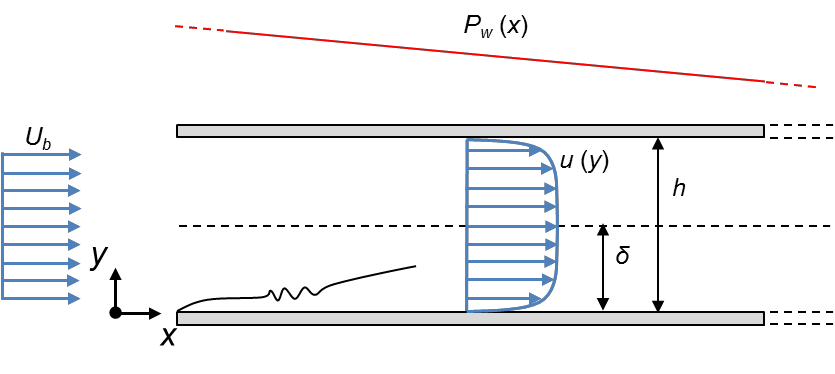
\includegraphics[width=\textwidth]{Sketch.png}
                \caption{Sketch of the test case}
                \label{fig:sketch}
        \end{figure}

\end{abstract}

\section{Introduction}
        \subsection{Flow Domain}

                The symmetry of the Reynolds-averaged flow can be exploited by solving over half of the system and imposing a symmetry condition on the half mid-plane (Figure~\ref{fig:domain}). As for the earlier test case, the inlet should not be placed in direct contact with the plate to avoid numerical issues at the bottom-left corner.

                \begin{figure}[ht!]
                        \centering
                        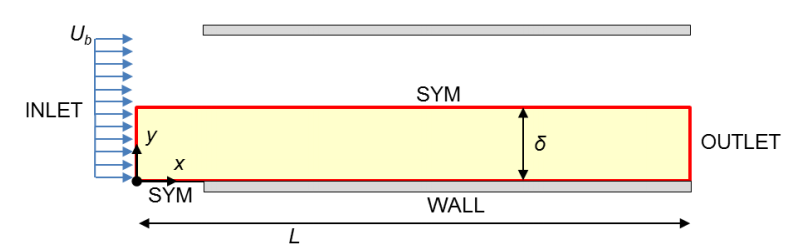
\includegraphics[width=\textwidth]{Domain.png}
                        \caption{Computational domain and boundary conditions}
                        \label{fig:domain}
                \end{figure}

                When defining the CFD model particular attention must be paid in choosing the proper boundary conditions, which are, in this case, inlet, outlet, solid walls and symmetry.

                \begin{itemize}
                        \item At the inlet, a uniform x-velocity profile equal to \( U_b \) is imposed, whereas the y-velocity and z-velocity components are specified as zero. No turbulence shall be assumed at the inlet boundary; this is achieved by setting an intensity \( TI \) equal to 0.
                        \item At the outlet, a zero external \( P^* \) is imposed. Note that the value of \( P^* \) at the outlet will not be zero owing to the presence of a finite outlet coefficient. In order to have \(P_{\text{outlet}}^* = P_{\text{ext}}^* = 0\), set the outlet coefficient to a very large value (e.g. \num{1e+10}). This is not really necessary, however.
                        \item At the solid walls, owing to the no-slip condition, the fluid velocity is zero. In the Finite Volume Framework with staggered-grid arrangement, only the y-velocity at the wall is imposed. The no-slip condition is imposed for the x-velocity indirectly. On the one hand, the advection flux of variable \( U \) through the near-wall cell faces is set to zero. On the other hand, the diffusion flux of variable \( U \) through the near-wall cell faces (that is, the wall shear force) is specified by obtaining the wall shear stress from the equilibrium wall function of Launder and Spalding. Note that the equilibrium wall function requires the dimensionless wall distance of the first grid nodes to be greater than 30 (and generally lower than about 130). Note that the dimensionless wall distance can be calculated only a posteriori.
                \end{itemize}
        
        \subsection{Data of the Problem}

                \begin{itemize}
                        \item Distance between the plates is \( h = \SI{1e-1}{\metre} \)
                        \item Bulk-mean velocity is \( U_b = \SI{1e0}{\metre \per \second} \)
                        \item Working fluid is water at \( \SI{2e1}{\celsius} \), treated as incompressible (\( \rho = \SI{9.9823e2}{\kilogram \per \metre \cubed} , \nu = \SI{1e-6}{\metre \squared \per \second} \))
                \end{itemize}
        
        \subsection{Report Structure}

                The remainder of the report is organized as follows: Section~\ref{sec:convergence} addresses the issue of Whole-Field residual convergence, Flow Full-Development and Grid Independence; Section~\ref{sec:qualitative} presents the relevant profiles and simulated scalars for the qualitative assesment of the model physical consistency; Section~\ref{sec:literature} compares the results of the simulation with the theoretical model studied during the lessons; finally, Section~\ref{sec:unstability} studies the behaviour of the CFD simulations when stability conditions (Extremely high Reynolds number/Over-refined wall mesh) are not met.

\section{Convergence of the CFD Solution} \label{sec:convergence}

        All simulations were ran setting up a minimum of 1000 iterations and a maximum of 10000, with a whole-field residual convergence criterion of 0.0001\%. The probe was set in the middle of the channel with respect to the start of the lower boundary plate. Additionally, regarding the grid-independence study, the near-wall cell width was reduced as much as possible while maintaining a \( y^+ \) value higher than 30, which turned out to be \( \SI{2e-3}{\metre} = \frac{\delta}{25} \).

\section{Qualitative assessment of the physical consistency of the CFD solution} \label{sec:qualitative}

        

\section{Comparison with literature models} \label{sec:literature}

        

\section{Optional questions for further individual study} \label{sec:unstability}

        

\bibliographystyle{abbrv}
\bibliography{main}

\end{document}
